\documentclass[tikz,border=5pt]{standalone}
\usepackage{times}
\usepackage{amsmath,amssymb}
\usepackage{pifont}
\newcommand{\cmark}{\ding{51}}%
\newcommand{\xmark}{\ding{55}}%
\usetikzlibrary{positioning,fit,arrows.meta,backgrounds,shapes.geometric,calc,shadows,decorations.pathreplacing}

\begin{document}
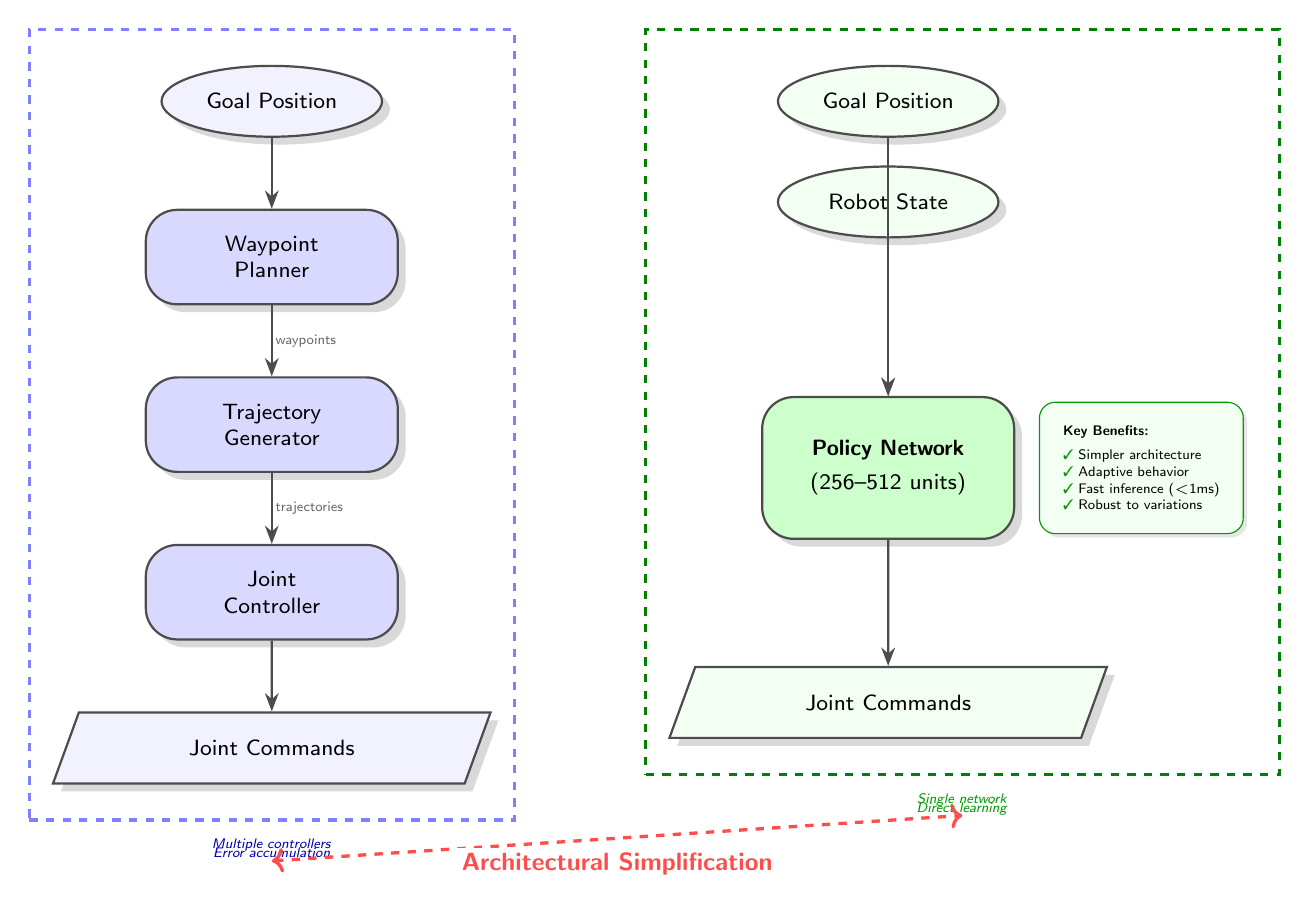
\begin{tikzpicture}[
    node distance=1cm and 3cm,
    % Enhanced module style with shadows
    module/.style={
        draw=black!70,
        rounded corners=4mm,
        minimum width=3.2cm,
        minimum height=1.2cm,
        font=\sffamily\footnotesize,
        fill=white,
        thick,
        align=center,
        drop shadow={opacity=0.3, shadow xshift=0.1cm, shadow yshift=-0.1cm}
    },
    % Enhanced input style
    input/.style={
        draw=black!70,
        ellipse,
        minimum width=2.8cm,
        minimum height=0.9cm,
        font=\sffamily\footnotesize,
        fill=white,
        thick,
        align=center,
        drop shadow={opacity=0.3, shadow xshift=0.1cm, shadow yshift=-0.1cm}
    },
    % Enhanced output style
    output/.style={
        draw=black!70,
        trapezium,
        trapezium left angle=70,
        trapezium right angle=110,
        minimum width=2.8cm,
        minimum height=0.9cm,
        font=\sffamily\footnotesize,
        fill=white,
        thick,
        align=center,
        drop shadow={opacity=0.3, shadow xshift=0.1cm, shadow yshift=-0.1cm}
    },
    % Arrow styles
    arrow/.style={->, >=Stealth, thick, color=black!70},
    arrow label/.style={font=\sffamily\tiny, color=black!60, midway, fill=white, inner sep=1pt},
    % Label and box styles
    label/.style={font=\sffamily\bfseries\normalsize},
    benefit box/.style={
        draw=green!60!black,
        rounded corners=2mm,
        fill=green!5,
        align=left,
        font=\sffamily\tiny,
        inner sep=0.3cm,
        drop shadow={opacity=0.2, shadow xshift=0.05cm, shadow yshift=-0.05cm}
    }
]

% Traditional Hierarchical Architecture (Left Side)
\node[input, fill=blue!5] (h_input) {Goal Position};
\node[module, below=0.9cm of h_input, fill=blue!15] (h_planner) {Waypoint\\Planner};
\node[module, below=0.9cm of h_planner, fill=blue!15] (h_traj) {Trajectory\\Generator};
\node[module, below=0.9cm of h_traj, fill=blue!15] (h_ctrl) {Joint\\Controller};
\node[output, below=0.9cm of h_ctrl, fill=blue!5] (h_output) {Joint Commands};

% Arrows for hierarchical with labels
\draw[arrow] (h_input) -- (h_planner);
\draw[arrow] (h_planner) -- node[arrow label, right] {waypoints} (h_traj);
\draw[arrow] (h_traj) -- node[arrow label, right] {trajectories} (h_ctrl);
\draw[arrow] (h_ctrl) -- (h_output);

% Bounding box for hierarchical
\node[draw=blue!50, dashed, very thick, fit=(h_input) (h_output), inner sep=0.45cm,
      label={[label, color=blue!70!black]above:Traditional Hierarchical}] (box_h) {};

% Add complexity annotation
\node[font=\sffamily\tiny, color=blue!70!black, below=0.1cm of box_h.south, align=center]
    {\textit{Multiple controllers}\\[-1mm]\textit{Error accumulation}};

% End-to-End Architecture (Right Side)
\node[input, right=5cm of h_input, fill=green!5] (e_input1) {Goal Position};
\node[input, below=0.35cm of e_input1, fill=green!5] (e_input2) {Robot State};
\node[module, below=2.0cm of e_input2, fill=green!20, minimum height=1.8cm, text width=2.8cm] (e_policy) {
    \textbf{Policy Network}\\[1mm]
    {\footnotesize (256--512 units)}
};
\node[output, below=1.6cm of e_policy, fill=green!5] (e_output) {Joint Commands};

% Arrows for end-to-end
\draw[arrow] (e_input1.south) -- ++(0,-0.15) -| (e_policy.north -| e_input1);
\draw[arrow] (e_input2.south) -- (e_policy.north -| e_input2);
\draw[arrow] (e_policy) -- (e_output);

% Enhanced benefits box
\node[benefit box, right=0.3cm of e_policy] (benefits) {
    \textbf{Key Benefits:}\\[1mm]
    \textcolor{green!60!black}{\cmark} Simpler architecture\\
    \textcolor{green!60!black}{\cmark} Adaptive behavior\\
    \textcolor{green!60!black}{\cmark} Fast inference ($<$1ms)\\
    \textcolor{green!60!black}{\cmark} Robust to variations
};

% Bounding box for end-to-end
\node[draw=green!50!black, dashed, very thick, fit=(e_input1) (e_output) (benefits), inner sep=0.45cm,
      label={[label, color=green!60!black]above:End-to-End (This Work)}] (box_e) {};

% Add simplicity annotation
\node[font=\sffamily\tiny, color=green!60!black, below=0.1cm of box_e.south, align=center]
    {\textit{Single network}\\[-1mm]\textit{Direct learning}};

% Comparison arrow with better styling
\draw[<->, very thick, dashed, red!70, line width=1.2pt]
    ([yshift=-0.5cm]box_h.south) --
    node[below=1mm, font=\sffamily\small\bfseries, color=red!70, fill=white, inner sep=2pt]
    {Architectural Simplification}
    ([yshift=-0.5cm]box_e.south);

\end{tikzpicture}
\end{document}
